\chapter{Mixing and Dissolving}\label{ch:g2:mixing-and-dissolving}

A sugar cube drops into a cup of hot tea. A spoon stirs, the cube
crumbles, and after a moment there is nothing left to see: the tea looks
exactly as it did before. Yet the tea now tastes sweet. The sugar has not
gone away --- it is hiding in the tea. This chapter is about putting
things together, and about the things that seem to vanish when we do.

\begin{omfigure}
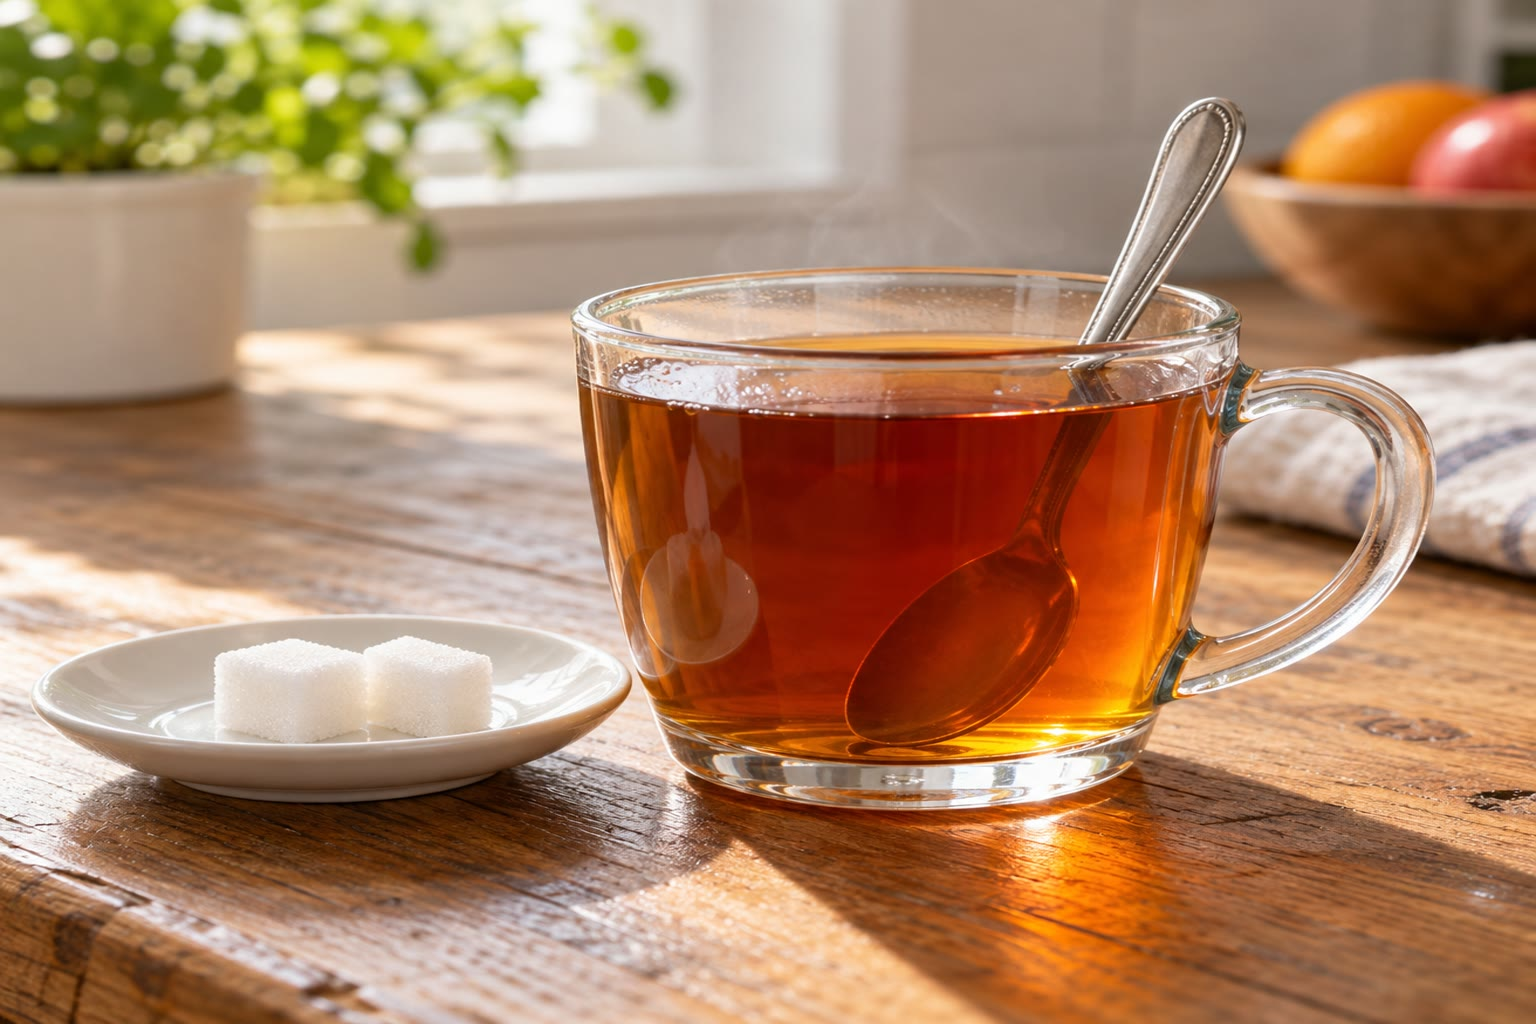
\includegraphics[width=0.55\linewidth]{images/book1/ai/g2-tea-sugar.jpg}

{\small A cup of tea and two sugar cubes. Stirred in, the sugar
disappears from sight, but not from the taste.}
\end{omfigure}

\section{Mixing things together}

\begin{definition}[Mixing]\label{def:g2:mixing-and-dissolving:mix}
To \emph{mix}\index{mix} is to put different things together, and often
to stir them. What we get is a mix of those things.
\end{definition}

\begin{example}[A bowl of muesli]\label{ex:g2:mixing-and-dissolving:muesli}
Oats, raisins, nuts and seeds are poured into one bowl: that is a \omterm{def:g2:mixing-and-dissolving:mix}{mix}.
Look closely and every ingredient can still be seen and picked out
again with the fingers --- a raisin stays a raisin, a nut stays a nut.
\end{example}

\begin{example}[Syrup in water]\label{ex:g2:mixing-and-dissolving:syrup}
Two liquids can be mixed too. Red syrup poured into a glass of water
sinks in curls of colour; after a stir, the whole glass is evenly pink.
The syrup and the water can no longer be told apart by eye.
\end{example}

\begin{omfigure}
\begin{minipage}[t]{0.48\linewidth}\centering
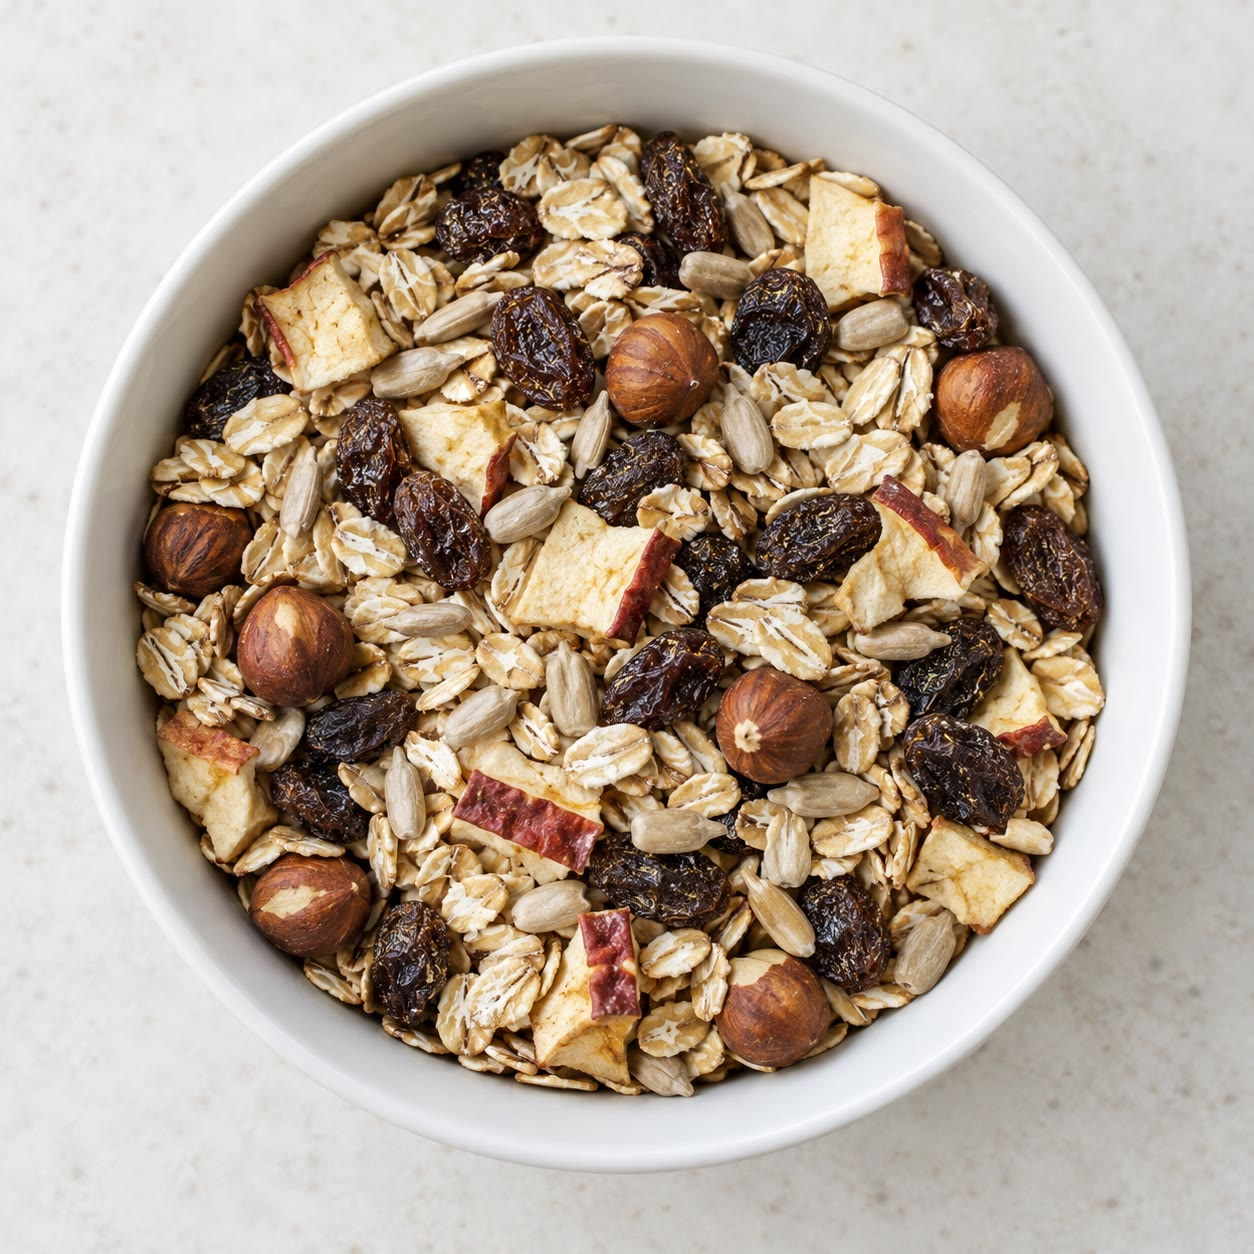
\includegraphics[width=\linewidth,height=4.6cm,keepaspectratio]{images/book1/ai/g2-muesli.jpg}

{\small Muesli: a \omterm{def:g2:mixing-and-dissolving:mix}{mix} in which every part can still be seen.}
\end{minipage}\hfill
\begin{minipage}[t]{0.48\linewidth}\centering
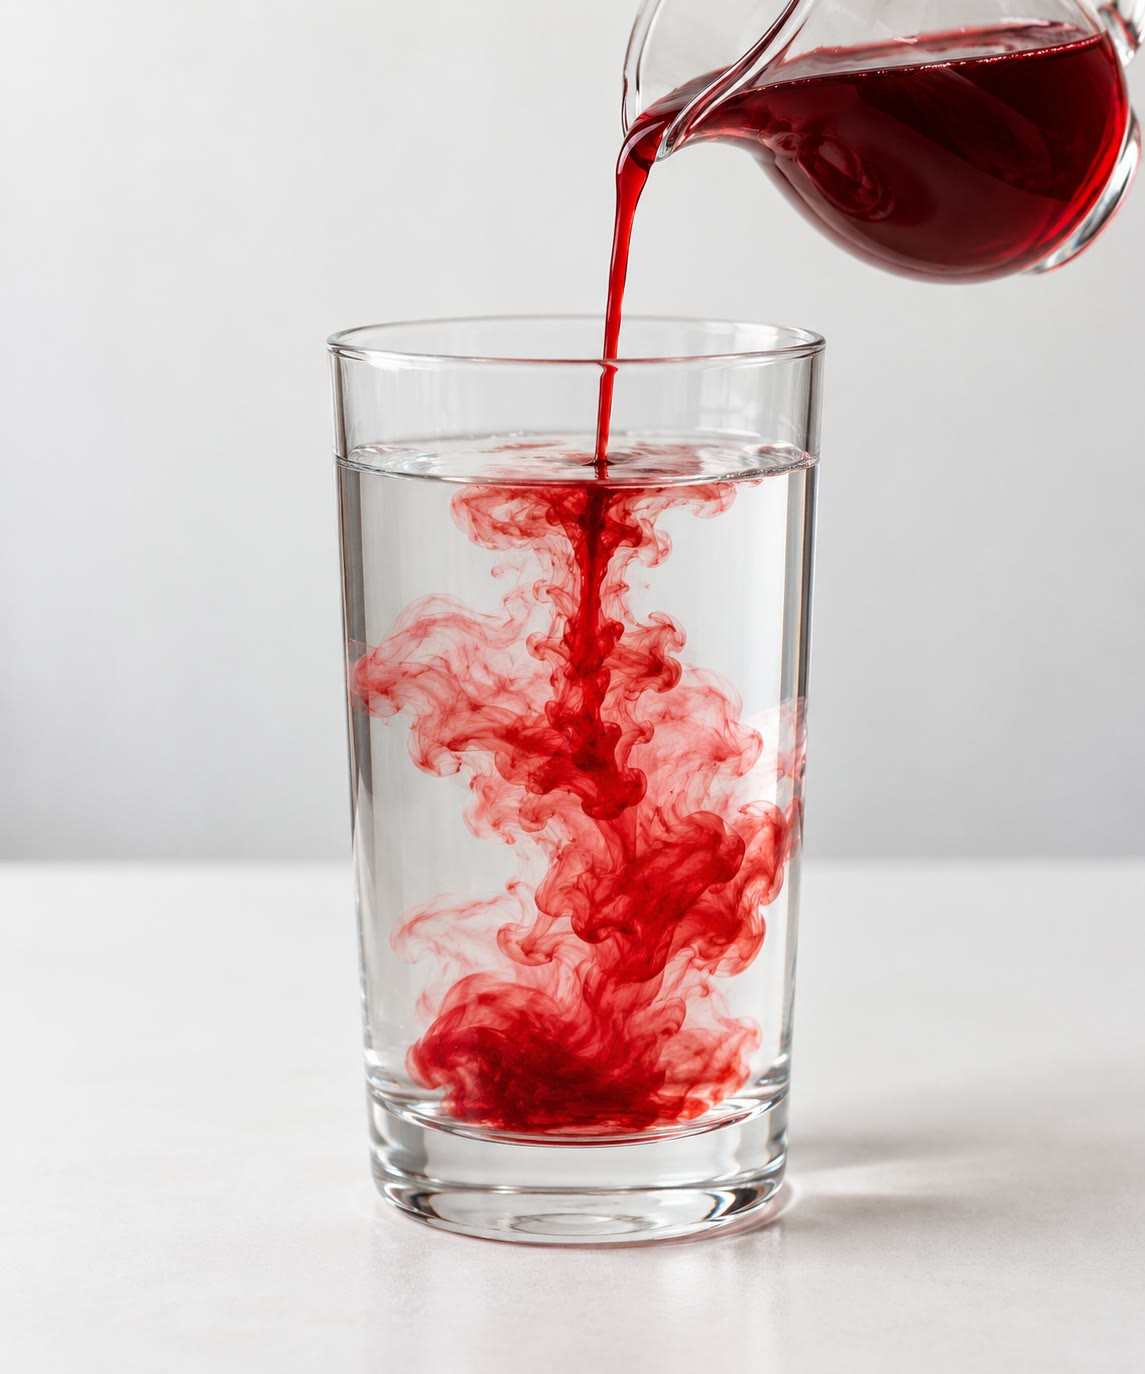
\includegraphics[width=\linewidth,height=4.6cm,keepaspectratio]{images/book1/ai/g2-syrup-in-water.jpg}

{\small Syrup poured into water: two liquids mixing.}
\end{minipage}
\end{omfigure}

\begin{remark}[Mixing destroys nothing]\label{rem:g2:mixing-and-dissolving:nothing-lost}
When things are mixed, nothing is lost and nothing new is made. The
oats, the raisins and the nuts are all still in the bowl. A later
chapter shows how to take a \omterm{def:g2:mixing-and-dissolving:mix}{mix} apart again.
\end{remark}

\section{Things that dissolve}

\begin{definition}[Dissolving and solution]\label{def:g2:mixing-and-dissolving:dissolve}
A solid \emph{dissolves}\index{dissolve} in water when, mixed into the
water and stirred, it disappears from sight and leaves the liquid
\emph{clear}, that is, see-through. Sugar and salt dissolve in water.
The clear liquid we obtain is called a
\emph{solution}\index{solution}: sugar water is a solution of sugar,
salty water a solution of salt.
\end{definition}

\begin{example}[A sugar cube in a glass of water]\label{ex:g2:mixing-and-dissolving:cube}
A sugar cube is placed at the bottom of a glass of still water. Its
corners soften, it grows smaller, and wavy streaks rise from it through
the water. If we stir, it is gone within a minute. If we do not stir, it
still disappears, only much more slowly.
\end{example}

\begin{remark}[Clear is not the same as colourless]\label{rem:g2:mixing-and-dissolving:clear}
Tea is brown and the syrup water is pink, but we can see through both:
they are clear. A \omterm{def:g2:mixing-and-dissolving:dissolve}{solution} can have a colour. What a \omterm{def:g2:mixing-and-dissolving:dissolve}{solution} never has
is bits floating in it or a layer at the bottom.
\end{remark}

\begin{method}[Does it dissolve?]\label{met:g2:mixing-and-dissolving:test}
To find out whether a solid \omterm{def:g2:mixing-and-dissolving:dissolve}{dissolves} in water:
\begin{enumerate}
  \item put a little of the solid into a glass of water;
  \item stir, then wait a few minutes;
  \item look through the glass:
    \begin{itemize}
      \item clear, and nothing at the bottom: the solid has dissolved;
      \item cloudy, or a layer at the bottom: the solid has not dissolved.
    \end{itemize}
\end{enumerate}
\end{method}

\section{Things that do not dissolve}

\begin{proposition}[Sand and chalk do not dissolve]\label{prop:g2:mixing-and-dissolving:not}
Many solids do not \omterm{def:g2:mixing-and-dissolving:dissolve}{dissolve} in water: sand, chalk, soil, pebbles,
flour. Stirred into water, they make it cloudy; left to rest, they sink
and settle at the bottom, and the water above becomes clearer again.
However long we stir, they never disappear.
\end{proposition}

\begin{example}[A jar of muddy water]\label{ex:g2:mixing-and-dissolving:mud}
Garden soil shaken in a jar of water turns it brown and cloudy. After an
hour the soil and the small pebbles lie in a dark layer at the bottom,
a few dead leaves float on top, and the water in between is only a
little cloudy. The soil has not dissolved.
\end{example}

\begin{omfigure}
\begin{minipage}[t]{0.48\linewidth}\centering
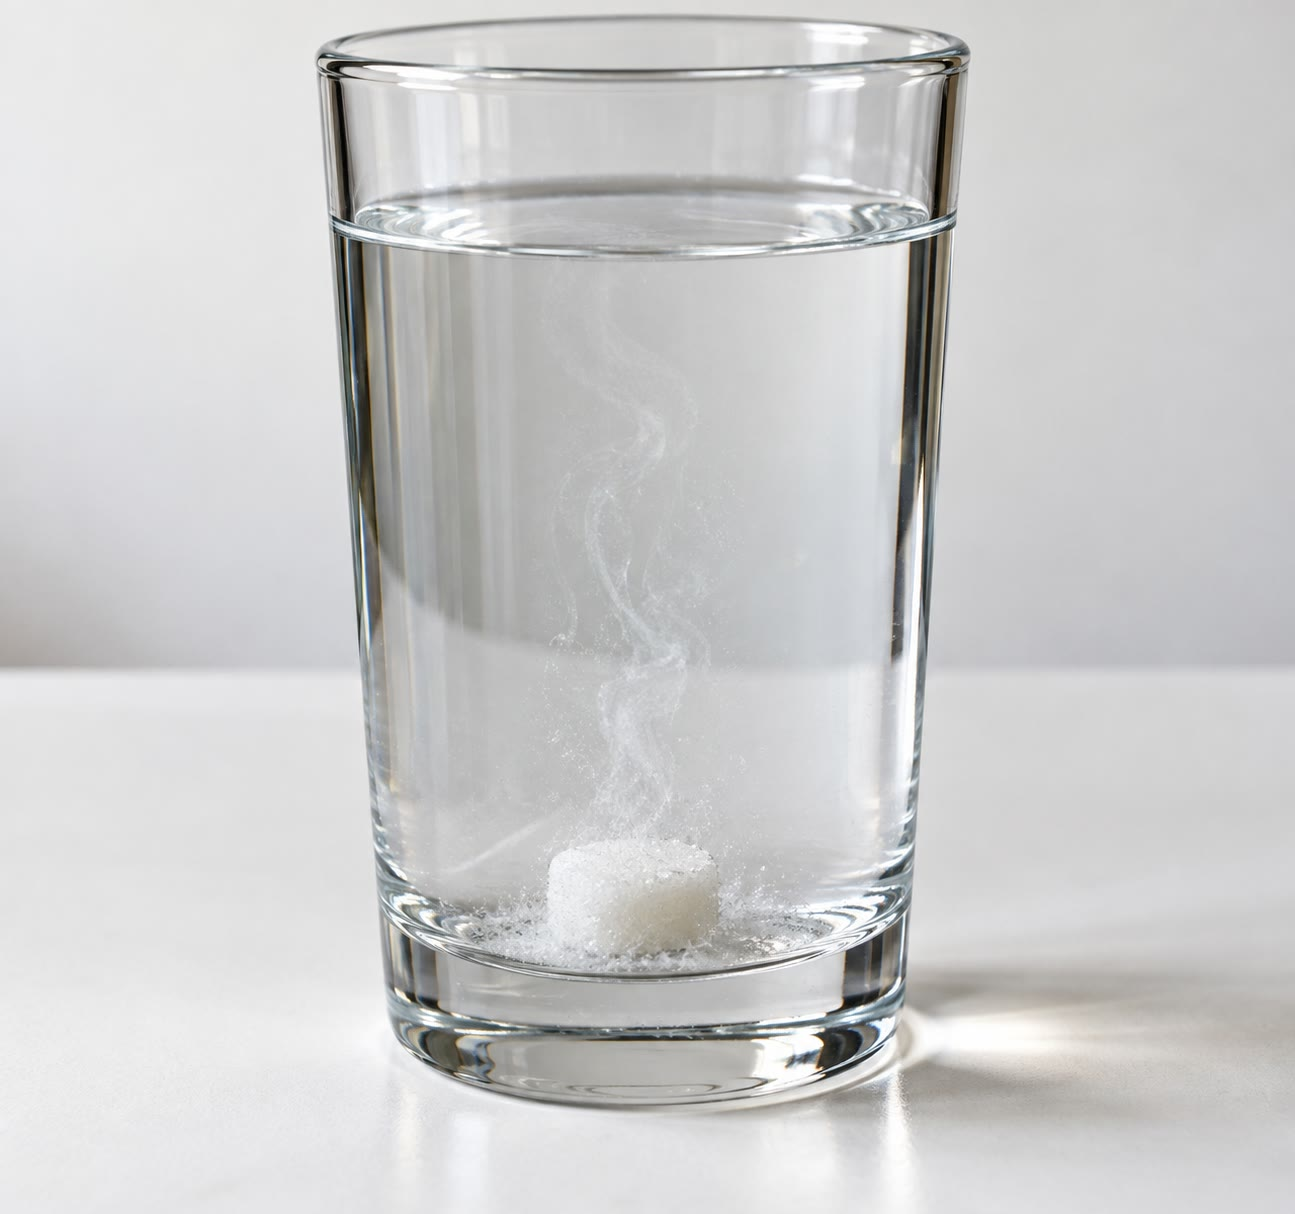
\includegraphics[width=\linewidth,height=4.6cm,keepaspectratio]{images/book1/ai/g2-sugar-cube-dissolving.jpg}

{\small Sugar dissolving: streaks rise from the cube.}
\end{minipage}\hfill
\begin{minipage}[t]{0.48\linewidth}\centering
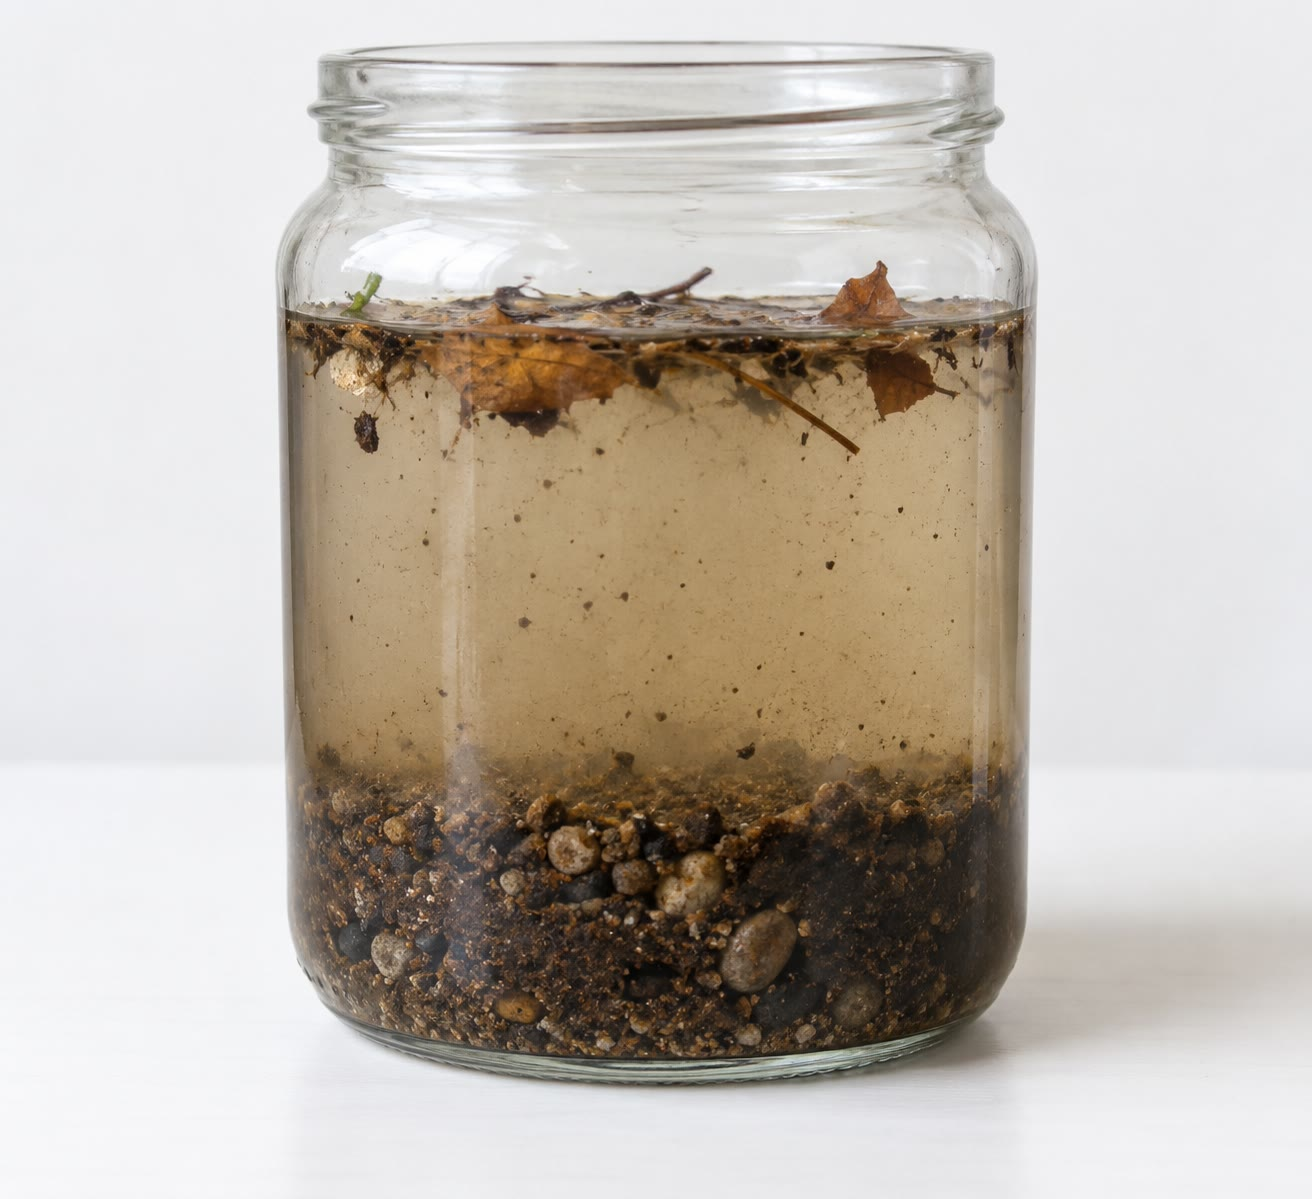
\includegraphics[width=\linewidth,height=4.6cm,keepaspectratio]{images/book1/ai/g2-muddy-jar.jpg}

{\small Soil does not \omterm{def:g2:mixing-and-dissolving:dissolve}{dissolve}: it settles at the bottom.}
\end{minipage}
\end{omfigure}

\begin{omfigure}
\begin{tikzpicture}[font=\small, scale=1.35]
  \pic[transform shape] at (0,0) {beaker={0.7}{omWater!70}};
  \fill[brown!55] (4.2,0) rectangle (5.8,0.22);
  \pic[transform shape] at (5,0) {beaker={0.7}{brown!12}};
  \fill[brown!55] (4.2,0) rectangle (5.8,0.22);
  \draw[omGlass, line width=0.7pt] (4.2,0.22) -- (4.2,0) -- (5.8,0) -- (5.8,0.22);
  \foreach \x/\y in {4.4/0.32,4.75/0.45,5.1/0.3,5.5/0.5,4.6/0.7,5.3/0.8,4.9/1.0}
    \fill[brown!60] (\x,\y) circle (0.025);
  \node[align=center, anchor=north] at (0,-0.15)
    {\textbf{sugar} in water, stirred:\\ clear, nothing at the bottom};
  \node[align=center, anchor=north] at (5,-0.15)
    {\textbf{sand} in water, stirred:\\ cloudy, a layer at the bottom};
  \draw[<-, omProp, thick] (6.0,0.11) -- (7.0,0.11)
    node[right, text=black] {the sand};
\end{tikzpicture}

{\small The test of \cref{met:g2:mixing-and-dissolving:test}: sugar
\omterm{def:g2:mixing-and-dissolving:dissolve}{dissolves}, sand does not.}
\end{omfigure}

\section{What dissolves is still there}

\begin{proposition}[A dissolved solid is still in the water]\label{prop:g2:mixing-and-dissolving:still-there}
When a solid \omterm{def:g2:mixing-and-dissolving:dissolve}{dissolves}, it does not vanish: it is spread all through the
water, in pieces far too small to be seen. Two clues show it is still
there:
\begin{itemize}
  \item sweet tea tastes sweet, and sea water tastes salty;
  \item when the water dries away, the solid is left behind.
\end{itemize}
\end{proposition}

\begin{remark}[No tasting in a laboratory]\label{rem:g2:mixing-and-dissolving:no-tasting}
We know that tea is sweet because tea is food. In a laboratory, nobody
ever tastes anything, not even a liquid that looks like water: the
second clue, letting the water dry away, is the one chemists use.
\end{remark}

\begin{example}[Salt from the sea]\label{ex:g2:mixing-and-dissolving:salt-pans}
On some sunny coasts, sea water is let into wide, shallow ponds. Day
after day the sun dries the water away. What remains on the bottom is
white salt, which is raked into heaps: the salt that was dissolved in
the sea. The salt on a dinner table often comes from such ponds.
\end{example}

\begin{omfigure}
\begin{tikzpicture}[font=\small, scale=1.25]
  % day 1: a saucer of salty water
  \fill[omWater!80] (0,0.18) ellipse (1.25 and 0.22);
  \draw[omGlass, line width=0.7pt] (-1.5,0.3) .. controls (-1.2,-0.15) and (1.2,-0.15) .. (1.5,0.3);
  \draw[omGlass, line width=0.5pt] (0,0.3) ellipse (1.5 and 0.28);
  \node[align=center, anchor=north] at (0,-0.35) {a saucer of\\ salty water};
  % the sun
  \fill[ocYellow] (3.4,1.45) circle (0.28);
  \foreach \a in {0,45,...,315}
    \draw[ocYellow!90!orange, thick] ($(3.4,1.45)+(\a:0.36)$) -- ($(3.4,1.45)+(\a:0.52)$);
  \draw[->, thick, omProp] (2.0,0.3) -- (4.8,0.3)
    node[midway, below, text=black, align=center] {a few sunny\\ days later};
  % later: a white crust
  \begin{scope}[xshift=6.3cm]
    \draw[omGlass, line width=0.7pt] (-1.5,0.3) .. controls (-1.2,-0.15) and (1.2,-0.15) .. (1.5,0.3);
    \draw[omGlass, line width=0.5pt] (0,0.3) ellipse (1.5 and 0.28);
    \foreach \x/\y in {-0.9/0.12,-0.6/0.2,-0.3/0.08,0/0.18,0.3/0.1,0.6/0.2,0.9/0.12,
                       -0.45/0.28,0.15/0.27,0.75/0.3,-0.75/0.31}
      \fill[white, draw=black!45, line width=0.2pt] (\x,\y) rectangle ++(0.11,0.07);
    \node[align=center, anchor=north] at (0,-0.35) {no water left:\\ white salt};
  \end{scope}
\end{tikzpicture}

{\small The water dries away; the salt that was dissolved in it stays
behind.}
\end{omfigure}

\begin{omfigure}
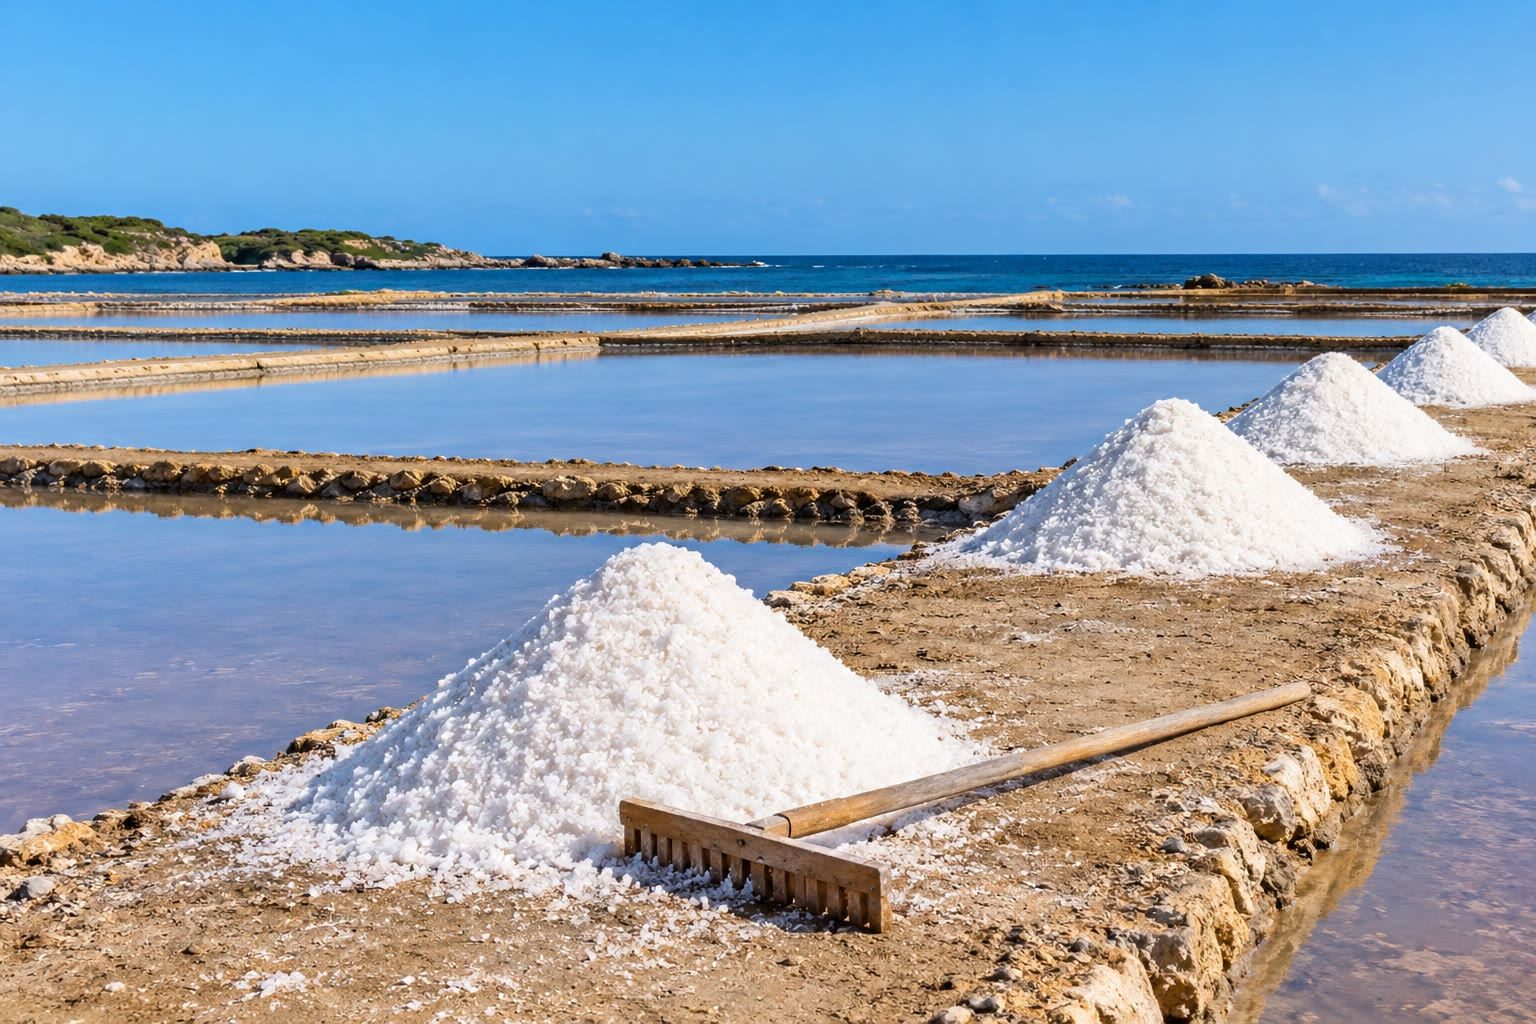
\includegraphics[width=0.62\linewidth]{images/book1/ai/g2-salt-pans.jpg}

{\small Salt ponds by the sea: the sun dries the water, the salt is
left in white heaps.}
\end{omfigure}

\begin{remark}[Dissolving is not melting]\label{rem:g2:mixing-and-dissolving:not-melting}
People often say that sugar ``melts'' in tea. It does not: melting is
what an ice cube does in the sun, turning into a liquid all by itself,
with no water needed. Sugar in tea needs the water, and the sugar is
still in it, spread out. The right word is \emph{\omterm{def:g2:mixing-and-dissolving:dissolve}{dissolves}}.
\end{remark}

\section{Exercises}

\begin{exercise}[$\star$]\label{exo:g2:mixing-and-dissolving:1}
Which of these solids \omterm{def:g2:mixing-and-dissolving:dissolve}{dissolve} in water, and which do not? Sugar,
sand, salt, chalk, pebbles.
\end{exercise}

\begin{exercise}[$\star$]\label{exo:g2:mixing-and-dissolving:2}
What is a \omterm{def:g2:mixing-and-dissolving:dissolve}{solution}? Give two examples from this chapter.
\end{exercise}

\begin{exercise}[$\star$]\label{exo:g2:mixing-and-dissolving:3}
Is a bowl of muesli a \omterm{def:g2:mixing-and-dissolving:mix}{mix}? Can you still see each of its parts?
\end{exercise}

\begin{exercise}[$\star$]\label{exo:g2:mixing-and-dissolving:4}
A white powder is stirred into a glass of water. After a few minutes,
the water is cloudy and a white layer has formed at the bottom. Has the
powder dissolved? Explain with
\cref{met:g2:mixing-and-dissolving:test}.
\end{exercise}

\begin{exercise}[$\star$]\label{exo:g2:mixing-and-dissolving:5}
A glass of syrup water is pink. Is it clear? Is it colourless? Is it a
\omterm{def:g2:mixing-and-dissolving:dissolve}{solution}?
\end{exercise}

\begin{exercise}[$\star$]\label{exo:g2:mixing-and-dissolving:6}
After stirring, no sugar can be seen in a cup of tea. Give the clue
that shows the sugar is still there.
\end{exercise}

\begin{exercise}[$\star$]\label{exo:g2:mixing-and-dissolving:7}
In the salt ponds, what does the sun take away, and what is left
behind?
\end{exercise}

\begin{exercise}[$\star$]\label{exo:g2:mixing-and-dissolving:8}
Tom says: ``The sugar melted in my tea.'' Which word should he use
instead, and why?
\end{exercise}

\begin{exercise}[$\star\star$]\label{exo:g2:mixing-and-dissolving:9}
Look at the figure with the two beakers. Without reading the words
under them, how can you tell which beaker holds the sand?
\end{exercise}

\begin{exercise}[$\star\star$]\label{exo:g2:mixing-and-dissolving:10}
A drop of tap water dries on a black plate and leaves a small white
ring. What does this tell us about tap water?
\end{exercise}

\begin{exercise}[$\star\star$]\label{exo:g2:mixing-and-dissolving:11}
In the laboratory, a teacher has two glasses of clear, colourless
liquid: one holds pure water, the other salty water. Nobody may taste
them. How can she find out which is which?
\end{exercise}
